\documentclass[__main__.tex]{subfiles}

\begin{document}

\qtitle{О}{08}
Принцип Гюйгенса-Френеля. Дифракционный интеграл. Пятно Пуассона-Араго.\\ 

Принцип Гюйгенса-Френеля. Дифракционный интеграл. Пятно Пуассона-Араго. Дифракционная решётка, её характеристики

\textbf{Принцип Гюйгенса-Френеля. }\\

\begin{figure}[h]
	\begin{center}
		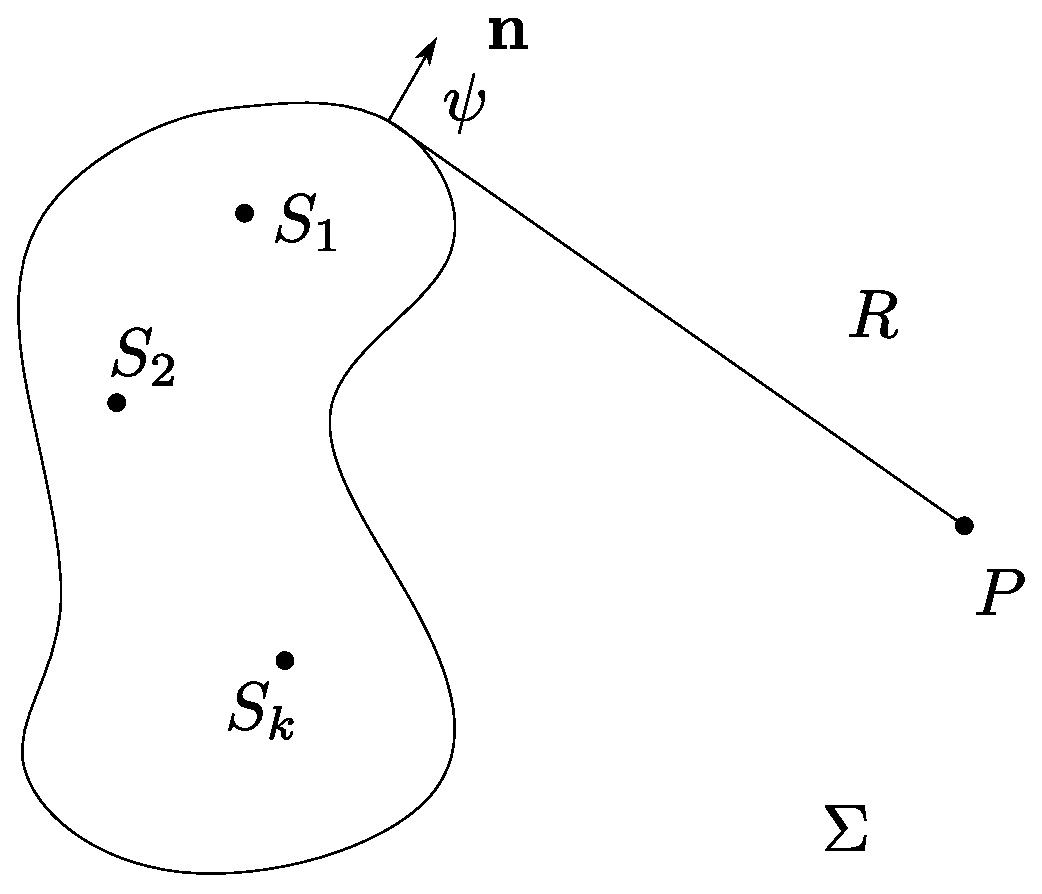
\includegraphics[width=0.5\linewidth]{img/o-08_1.eps}
	\end{center}
\end{figure}

1. Если окружить систему когерентных источников произвольной замкнутой поверхностью $\Sigma$, то каждую точку этой поверхности можно считать источником вторичных когерентных сферических волн, распространяющихся по всем направлениям. Амплитуда этих волн на поверхности находится как суперпозиция волн, идущих от первичных источников. Световое поле в любой точке вне этой поверхности можно рассчитывать как суперпозицию всех вторичных волн. 

2. Если часть этой поверхности закрыта непрозрачным экраном, то учитывать нужно только волны, идущие от открытых частей поверхности.\\

Обе эти части принципа объединяет \textbf{дифракционный интеграл Релея}:
$$E(P) = \frac{1}{i\lambda}\iint\limits_{\Sigma'} \widetilde K(\psi) E(Q)\frac{e^{ikR}}{R}d\sigma,$$
где $\Sigma'$ - открытая часть поверхности $\Sigma$, $Q$ - точка на $\Sigma'$, $E(Q)\frac{e^{ikR}}{R}$ - сферическая волна, идущая от этой точки\\ 

\textbf{Пятно Пуассон-Араго с объяснением появления}\\

Начнем с метода, примененного Френелем:\\

1.Если окружить систему когерентных источников произвольной замкнутой поверхностью $\Sigma$, то каждую точку этой поверхности можно считать источником вторичных когерентных сферических волн, распростроняющихся по всем направлениям. Амплитуда этих волн на поверхности находится как суперпозиция волн, идущих от первичных источников. Светлое поле в любой точке $P$ вне этой поверхности можно расчитывать как суперпозицию всех вторичных волн.\\
%%пикча из лекций братишки, стр 5

2.Если часть этой поверхности закрыта непрозрачным экраном, то учитывать нужно только волны, идущие от открытых частей поверхности.\\

Обе эти части объеденяет интеграл Рэлея:
\begin{gather}
E(P)= \frac{1}{i\lambda}\iint_{\Sigma'} \tilde{K}(\xi)E(Q)\frac{e^{ikR}}{R}d\sigma ,
\end{gather}

Здесь $\Sigma'$ - открытая часть поверхности $\Sigma$, $Q$ - точка на $\Sigma'$. $E(Q)=\frac{e^{ikR}}{R}$ -сферическая волна, идущая от этой точки, причем ее амплитуда $E(Q)$ - световое поле в этой точке, создаваемое первичными источниками, $d\sigma$ - элемент поверхности $\Sigma$. Функция $\tilde{K}(\xi)$ медленно меняется от единицы при $\xi = 0$ (на передней, ближайшей к точке $P$, части замкнутой поверхности) до нуля при $\xi = \pi$(на противоположной стороне поверхности).\\

Множитель $\frac{1}{i} $ перед интегралом говорит о том, что вторичные волны опережают приходящие от источника по фазе на $\frac{\pi}{2}$.\\
%%пикча глазика из лекций братишки

Рассмотрим простейший случай - поле от точечного источника $S$ в точке наблюдения $P$, когда все препятствия симметричны относительно оси $SP$. Таковыми на рисунке являются диафрагма $D_1$ и непрозрачный кружок $D_2$. Вспомогательной поверхностью служит сфера $\Sigma$ радиуса $\rho$. Расстояние от этой сферы до точки $P$ будем обозночать $R_0$.\\

На открытом участке текущее значение растояния $R$ от вторичного источника на сфере до точки $P$ меняется $R_{min}$ до $R_{max}$, а угол $\theta$ - от $\theta_{min}$ до $\theta_{max}$.\\

От источника $S$ распространяется сферическая волна, и на сфере она принимает вид $E(Q)=\frac{E_s e^{ikp}}{\rho}$. После интегрирования по углу $\phi$ сферической системы координат с центром в точке $S$ интеграл по открытой части поверхности принимает вид:\\
\begin{gather}
E(P)=\frac{2\pi}{i\lambda} \int_{\theta_{min}}^{\theta_{max}} \tilde{K} (\xi) \frac{E_S e^{ik\rho}}{\rho} \frac{e^{ikR}}{R} \rho^2 \sin(\theta) d\theta ,
\end{gather}

Пререйдем в этом интеграле от переменной $\theta$ к переменной $R$.\\
Из треугольника $SQP$ по теореме косинусов имеем:
\begin{gather}
R^2 = \rho^2 + (\rho + R_0)^2 - 2\rho(\rho + R_0)\cos(\theta) ,
\end{gather}
и берем дифференциал от левой и правой части
\begin{gather}
2RdR = 2\rho(\rho + R_0)\sin(\theta)d\theta ,
\end{gather}
и подставляем $\sin (\theta) = \frac{RdR}{\rho(\rho + R_0)}$ в интеграл :
\begin{gather}
E(P) = \frac{2\pi E_S e^{ik(\rho + R_0)}}{i\lambda(\rho + R_0)} \int_{R_{min}}^{R_{max}} K(R)e^{ik(R-R_0)}dR ,
\end{gather}

Функция $K(R)$ - это то, во что перешла функция $\tilde{K}(\xi)$ при сделанной замене переменных. Ее явный вид для нас не очень важен. Подчеркнем только, что она медленно и монотонно меняется от еденицы до нудя, причем:
\begin{gather}
K(R_0) = 1 , \\
K(R_0+2\rho) = 0 ,
\end{gather}

Дополнительно вынесли за интеграл множитель $\frac{e^{ikR_0}}{R_0}$, чтобы выделить величину:
\begin{gather}
E_0 = \frac{E_S e^{ik(\rho + R_0)}}{\rho + R_0} ,
\end{gather}
имеющую очевидный физический смысл: это сферическая волна от первичного источника $S$, пришедшая в точку наблюдения $P$, т.е. поле в этой точке в отсутствие каких либо преград.\\

К интегралу в формуле (0.5)
применим нашу рабочую формулу
\begin{gather}
\int_{a}^{b} f(x)e^{ikx}dx \approx \frac{1}{ik} (f(b)e^{ikb} - f(a)e^{ika}) ,
\end{gather}
и получим:
\begin{gather}
\int_{R{min}}^{R{max}} K(R)e^{ik(R-R_0)}dR = \frac{1}{ik}(K(R_{max})e^{ik(R_{max} - R_0)}-K(R_{min}e^{ik(R_{min} - R_0)})) ,
\end{gather}

Подставим (0.8) и (0.10)
в соотношение (0.5)
и окончательно получаем ($E(P)=E$)\\
\begin{gather}
E = E_0 (K(R_{min})e^{ik(R_{min} - R_0)}-K(R_{max}e^{ik(R_{max} - R_0)})) ,
\end{gather}

Пусть $I_0 = E_0 E_0*$ - интенсивность вточке наблюдения вотсутствие преград, тогда интенсивность в точки наблюдения записывается так:
\begin{gather}
I = I_0 ((K(R_{min})))^2 +(K(R_{max}))^2 - 2K(R_{min})K(R_{max})\cos(k(R_{max}-R_{min})) ,
\end{gather}

Сначала проверим, что наша формула (0.11)
дает правельный результат в отсутвие препятствий. В этом случае $R_{min} = R_0$ и $R_{max} = R_0 + 2\rho$, так что согласно условиям (0.6) и (0.7)
\begin{gather}
K(R_{min}) = 1 ,\\
K(R_{max}) = 0 ,
\end{gather}
и $E = E_0$, как и должно быть.
Теперь уберем диафрагму и оставим только кружок $D_2$, перекрывающий осевые лучи. В этом случае $K(R_{max}) = 0$ и $E=E_0 K(R_{min})e^{ik(R_{min}-R_0)}$, в для интенсивности $I \sim EE*$ получаем $I = I_0 (K(R_{min}))^2$, т.е. если прегродить прямой путь к точке наблюдения, то за преградой всегда будет светлое пятно. Этот эффект называется пятном Араго-Пуассона.\\

\end{document}